\documentclass[twoside]{book}

% Packages required by doxygen
\usepackage{fixltx2e}
\usepackage{calc}
\usepackage{doxygen}
\usepackage[export]{adjustbox} % also loads graphicx
\usepackage{graphicx}
\usepackage[utf8]{inputenc}
\usepackage{makeidx}
\usepackage{multicol}
\usepackage{multirow}
\PassOptionsToPackage{warn}{textcomp}
\usepackage{textcomp}
\usepackage[nointegrals]{wasysym}
\usepackage[table]{xcolor}

% Font selection
\usepackage[T1]{fontenc}
\usepackage[scaled=.90]{helvet}
\usepackage{courier}
\usepackage{amssymb}
\usepackage{sectsty}
\renewcommand{\familydefault}{\sfdefault}
\allsectionsfont{%
  \fontseries{bc}\selectfont%
  \color{darkgray}%
}
\renewcommand{\DoxyLabelFont}{%
  \fontseries{bc}\selectfont%
  \color{darkgray}%
}
\newcommand{\+}{\discretionary{\mbox{\scriptsize$\hookleftarrow$}}{}{}}

% Page & text layout
\usepackage{geometry}
\geometry{%
  a4paper,%
  top=2.5cm,%
  bottom=2.5cm,%
  left=2.5cm,%
  right=2.5cm%
}
\tolerance=750
\hfuzz=15pt
\hbadness=750
\setlength{\emergencystretch}{15pt}
\setlength{\parindent}{0cm}
\setlength{\parskip}{3ex plus 2ex minus 2ex}
\makeatletter
\renewcommand{\paragraph}{%
  \@startsection{paragraph}{4}{0ex}{-1.0ex}{1.0ex}{%
    \normalfont\normalsize\bfseries\SS@parafont%
  }%
}
\renewcommand{\subparagraph}{%
  \@startsection{subparagraph}{5}{0ex}{-1.0ex}{1.0ex}{%
    \normalfont\normalsize\bfseries\SS@subparafont%
  }%
}
\makeatother

% Headers & footers
\usepackage{fancyhdr}
\pagestyle{fancyplain}
\fancyhead[LE]{\fancyplain{}{\bfseries\thepage}}
\fancyhead[CE]{\fancyplain{}{}}
\fancyhead[RE]{\fancyplain{}{\bfseries\leftmark}}
\fancyhead[LO]{\fancyplain{}{\bfseries\rightmark}}
\fancyhead[CO]{\fancyplain{}{}}
\fancyhead[RO]{\fancyplain{}{\bfseries\thepage}}
\fancyfoot[LE]{\fancyplain{}{}}
\fancyfoot[CE]{\fancyplain{}{}}
\fancyfoot[RE]{\fancyplain{}{\bfseries\scriptsize Generated by Doxygen }}
\fancyfoot[LO]{\fancyplain{}{\bfseries\scriptsize Generated by Doxygen }}
\fancyfoot[CO]{\fancyplain{}{}}
\fancyfoot[RO]{\fancyplain{}{}}
\renewcommand{\footrulewidth}{0.4pt}
\renewcommand{\chaptermark}[1]{%
  \markboth{#1}{}%
}
\renewcommand{\sectionmark}[1]{%
  \markright{\thesection\ #1}%
}

% Indices & bibliography
\usepackage{natbib}
\usepackage[titles]{tocloft}
\setcounter{tocdepth}{3}
\setcounter{secnumdepth}{5}
\makeindex

% Hyperlinks (required, but should be loaded last)
\usepackage{ifpdf}
\ifpdf
  \usepackage[pdftex,pagebackref=true]{hyperref}
\else
  \usepackage[ps2pdf,pagebackref=true]{hyperref}
\fi
\hypersetup{%
  colorlinks=true,%
  linkcolor=blue,%
  citecolor=blue,%
  unicode%
}

% Custom commands
\newcommand{\clearemptydoublepage}{%
  \newpage{\pagestyle{empty}\cleardoublepage}%
}

\usepackage{caption}
\captionsetup{labelsep=space,justification=centering,font={bf},singlelinecheck=off,skip=4pt,position=top}

%===== C O N T E N T S =====

\begin{document}

% Titlepage & ToC
\hypersetup{pageanchor=false,
             bookmarksnumbered=true,
             pdfencoding=unicode
            }
\pagenumbering{alph}
\begin{titlepage}
\vspace*{7cm}
\begin{center}%
{\Large Aqua\+Engine }\\
\vspace*{1cm}
{\large Generated by Doxygen 1.8.12}\\
\end{center}
\end{titlepage}
\clearemptydoublepage
\pagenumbering{roman}
\tableofcontents
\clearemptydoublepage
\pagenumbering{arabic}
\hypersetup{pageanchor=true}

%--- Begin generated contents ---
\chapter{Hierarchical Index}
\section{Class Hierarchy}
This inheritance list is sorted roughly, but not completely, alphabetically\+:\begin{DoxyCompactList}
\item \contentsline{section}{ae\+:\+:Application}{\pageref{classae_1_1_application}}{}
\item bitset\begin{DoxyCompactList}
\item \contentsline{section}{ae\+:\+:error\+:\+:Flags}{\pageref{structae_1_1error_1_1_flags}}{}
\end{DoxyCompactList}
\item \contentsline{section}{ae\+:\+:Error}{\pageref{classae_1_1_error}}{}
\begin{DoxyCompactList}
\item \contentsline{section}{My\+Error}{\pageref{class_my_error}}{}
\end{DoxyCompactList}
\item \contentsline{section}{ae\+:\+:Instance}{\pageref{classae_1_1_instance}}{}
\item Test\begin{DoxyCompactList}
\item \contentsline{section}{Application\+Test}{\pageref{class_application_test}}{}
\item \contentsline{section}{Error\+Flags\+Test}{\pageref{class_error_flags_test}}{}
\item \contentsline{section}{Error\+Test}{\pageref{class_error_test}}{}
\item \contentsline{section}{Error\+Vulkan\+Test}{\pageref{class_error_vulkan_test}}{}
\item \contentsline{section}{Instance\+Test}{\pageref{class_instance_test}}{}
\item \contentsline{section}{Window\+Test}{\pageref{class_window_test}}{}
\end{DoxyCompactList}
\item Window\begin{DoxyCompactList}
\item \contentsline{section}{ae\+:\+:G\+L\+FW}{\pageref{classae_1_1_g_l_f_w}}{}
\end{DoxyCompactList}
\end{DoxyCompactList}

\chapter{Class Index}
\section{Class List}
Here are the classes, structs, unions and interfaces with brief descriptions\+:\begin{DoxyCompactList}
\item\contentsline{section}{\hyperlink{classae_1_1_application}{ae\+::\+Application} \\*Base class to create Aqua\+Engine application }{\pageref{classae_1_1_application}}{}
\item\contentsline{section}{\hyperlink{class_application_test}{Application\+Test} }{\pageref{class_application_test}}{}
\item\contentsline{section}{\hyperlink{classae_1_1_error}{ae\+::\+Error} \\*Handle errors }{\pageref{classae_1_1_error}}{}
\item\contentsline{section}{\hyperlink{class_error_flags_test}{Error\+Flags\+Test} }{\pageref{class_error_flags_test}}{}
\item\contentsline{section}{\hyperlink{class_error_test}{Error\+Test} }{\pageref{class_error_test}}{}
\item\contentsline{section}{\hyperlink{class_error_vulkan_test}{Error\+Vulkan\+Test} }{\pageref{class_error_vulkan_test}}{}
\item\contentsline{section}{\hyperlink{structae_1_1error_1_1_flags}{ae\+::error\+::\+Flags} }{\pageref{structae_1_1error_1_1_flags}}{}
\item\contentsline{section}{\hyperlink{classae_1_1_g_l_f_w}{ae\+::\+G\+L\+FW} }{\pageref{classae_1_1_g_l_f_w}}{}
\item\contentsline{section}{\hyperlink{classae_1_1_instance}{ae\+::\+Instance} }{\pageref{classae_1_1_instance}}{}
\item\contentsline{section}{\hyperlink{class_instance_test}{Instance\+Test} }{\pageref{class_instance_test}}{}
\item\contentsline{section}{\hyperlink{class_my_error}{My\+Error} }{\pageref{class_my_error}}{}
\item\contentsline{section}{\hyperlink{classae_1_1_singleton}{ae\+::\+Singleton$<$ T $>$} }{\pageref{classae_1_1_singleton}}{}
\item\contentsline{section}{\hyperlink{classae_1_1error_1_1_vulkan}{ae\+::error\+::\+Vulkan} }{\pageref{classae_1_1error_1_1_vulkan}}{}
\item\contentsline{section}{\hyperlink{classae_1_1_window}{ae\+::\+Window} }{\pageref{classae_1_1_window}}{}
\item\contentsline{section}{\hyperlink{class_window_test}{Window\+Test} }{\pageref{class_window_test}}{}
\end{DoxyCompactList}

\chapter{Class Documentation}
\hypertarget{classae_1_1_application}{}\section{ae\+:\+:Application Class Reference}
\label{classae_1_1_application}\index{ae\+::\+Application@{ae\+::\+Application}}


Base class to create Aqua\+Engine application.  




{\ttfamily \#include $<$application.\+h$>$}

\subsection*{Public Member Functions}
\begin{DoxyCompactItemize}
\item 
\hypertarget{classae_1_1_application_a7e9a30ce07057f5f37b02500f876436a}{}\label{classae_1_1_application_a7e9a30ce07057f5f37b02500f876436a} 
{\bfseries Application} (const \hyperlink{classae_1_1_application}{Application} \&)=delete
\item 
\hypertarget{classae_1_1_application_ae18f573dfd5d579e562784781f53a87a}{}\label{classae_1_1_application_ae18f573dfd5d579e562784781f53a87a} 
\hyperlink{classae_1_1_application}{Application} \& {\bfseries operator=} (const \hyperlink{classae_1_1_application}{Application} \&)=delete
\item 
\hypertarget{classae_1_1_application_ac5803ae7a946ba88cb65a110c9ae6621}{}\label{classae_1_1_application_ac5803ae7a946ba88cb65a110c9ae6621} 
\hyperlink{classae_1_1_application}{Application} \& {\bfseries operator=} (\hyperlink{classae_1_1_application}{Application} \&\&)=delete
\item 
\hypertarget{classae_1_1_application_a4c0b8e813b5596a08ecf5f69423fda99}{}\label{classae_1_1_application_a4c0b8e813b5596a08ecf5f69423fda99} 
{\bfseries Application} (\hyperlink{classae_1_1_application}{Application} \&\&)=delete
\item 
\hypertarget{classae_1_1_application_a2f4107e93f0e3c2525ad65f70a951fed}{}\label{classae_1_1_application_a2f4107e93f0e3c2525ad65f70a951fed} 
std\+::string \hyperlink{classae_1_1_application_a2f4107e93f0e3c2525ad65f70a951fed}{name} () const noexcept
\begin{DoxyCompactList}\small\item\em Returns a copy of the application name. \end{DoxyCompactList}\item 
\hypertarget{classae_1_1_application_aa83e498302067740788c8e3bd9b95a62}{}\label{classae_1_1_application_aa83e498302067740788c8e3bd9b95a62} 
void \hyperlink{classae_1_1_application_aa83e498302067740788c8e3bd9b95a62}{set\+\_\+name} (std\+::string) noexcept
\begin{DoxyCompactList}\small\item\em Set the application name. \end{DoxyCompactList}\item 
\hypertarget{classae_1_1_application_a7b6d08a1968612f523e6f6c3b2c7786b}{}\label{classae_1_1_application_a7b6d08a1968612f523e6f6c3b2c7786b} 
int \hyperlink{classae_1_1_application_a7b6d08a1968612f523e6f6c3b2c7786b}{version} () const noexcept
\begin{DoxyCompactList}\small\item\em Returns a copy of the application versions. \end{DoxyCompactList}\item 
\hypertarget{classae_1_1_application_a7911bcd7ef75ee1bdce9d783b5d9577b}{}\label{classae_1_1_application_a7911bcd7ef75ee1bdce9d783b5d9577b} 
void \hyperlink{classae_1_1_application_a7911bcd7ef75ee1bdce9d783b5d9577b}{set\+\_\+version} (const int) noexcept
\begin{DoxyCompactList}\small\item\em Set the application version with integer. \end{DoxyCompactList}\item 
\hypertarget{classae_1_1_application_aa9c90bf2ce938a0861254f9ed656a68f}{}\label{classae_1_1_application_aa9c90bf2ce938a0861254f9ed656a68f} 
void \hyperlink{classae_1_1_application_aa9c90bf2ce938a0861254f9ed656a68f}{set\+\_\+version} (const int major, const int minor, const int patch) noexcept
\begin{DoxyCompactList}\small\item\em Helper to set the application version. \end{DoxyCompactList}\item 
\hypertarget{classae_1_1_application_a430877054b3f5cb743b3d8541a0a37e8}{}\label{classae_1_1_application_a430877054b3f5cb743b3d8541a0a37e8} 
const std\+::shared\+\_\+ptr$<$ Vk\+Application\+Info $>$ \hyperlink{classae_1_1_application_a430877054b3f5cb743b3d8541a0a37e8}{informations} () const noexcept
\begin{DoxyCompactList}\small\item\em Returns smart-\/pointer of Vulkan informations. \end{DoxyCompactList}\end{DoxyCompactItemize}
\subsection*{Static Public Attributes}
\begin{DoxyCompactItemize}
\item 
static const Vk\+Application\+Info \hyperlink{classae_1_1_application_a4c12a034bcd9b22ebe2c8770e62f9792}{k\+Default\+Informations}
\begin{DoxyCompactList}\small\item\em Base populated informations. \end{DoxyCompactList}\end{DoxyCompactItemize}


\subsection{Detailed Description}
Base class to create Aqua\+Engine application. 

Example \+:


\begin{DoxyCode}
\textcolor{keyword}{class }DemoApp : \textcolor{keyword}{public} \hyperlink{classae_1_1_application}{ae::Application} \{
    DemoApp();
    \textcolor{keyword}{virtual} ~DemoApp();

   \textcolor{keyword}{protected}:
    std::shared\_ptr<ae::error::Vulkan> error\_vulkan\_\{
        std::make\_shared<ae::error::Vulkan>()\};
    std::shared\_ptr<ae::Instance> instance\_\{
    std::make\_shared<ae::Instance>()\};
    std::unique\_ptr<ae::Window> window\_\{ae::Window::Create()\};
\};

DemoApp::DemoApp() : \hyperlink{namespaceae}{ae}::Application() \{
    set\_name(\textcolor{stringliteral}{"Demo AquaEngine"});
    set\_version(1, 0, 0);
    error\_vulkan\_->set\_instance(instance\_);
    instance\_->AddExtensions(window\_->extensions());

    error\_vulkan\_->set\_result(instance\_->Create());
    \textcolor{keywordflow}{if} (error\_vulkan\_->IsError()) \textcolor{keywordflow}{throw} error\_vulkan\_->Message();

    \textcolor{keywordflow}{while} (window\_->PoolEvent()) \{
    \};
\}

DemoApp::~DemoApp() \{\}
\end{DoxyCode}
 

\subsection{Member Data Documentation}
\hypertarget{classae_1_1_application_a4c12a034bcd9b22ebe2c8770e62f9792}{}\label{classae_1_1_application_a4c12a034bcd9b22ebe2c8770e62f9792} 
\index{ae\+::\+Application@{ae\+::\+Application}!k\+Default\+Informations@{k\+Default\+Informations}}
\index{k\+Default\+Informations@{k\+Default\+Informations}!ae\+::\+Application@{ae\+::\+Application}}
\subsubsection{\texorpdfstring{k\+Default\+Informations}{kDefaultInformations}}
{\footnotesize\ttfamily const Vk\+Application\+Info ae\+::\+Application\+::k\+Default\+Informations\hspace{0.3cm}{\ttfamily [inline]}, {\ttfamily [static]}}

{\bfseries Initial value\+:}
\begin{DoxyCode}
\{
        VK\_STRUCTURE\_TYPE\_APPLICATION\_INFO,
        \textcolor{keyword}{nullptr},
        \textcolor{stringliteral}{""},
        MakeVersion(1, 0, 0),
        \textcolor{stringliteral}{"AquaEngine"},
        MakeVersion(1, 0, 0),
        VK\_API\_VERSION\_1\_0\}
\end{DoxyCode}


Base populated informations. 



The documentation for this class was generated from the following files\+:\begin{DoxyCompactItemize}
\item 
src/application.\+h\item 
src/application.\+cc\end{DoxyCompactItemize}

\hypertarget{class_application_test}{}\section{Application\+Test Class Reference}
\label{class_application_test}\index{Application\+Test@{Application\+Test}}


Inheritance diagram for Application\+Test\+:\nopagebreak
\begin{figure}[H]
\begin{center}
\leavevmode
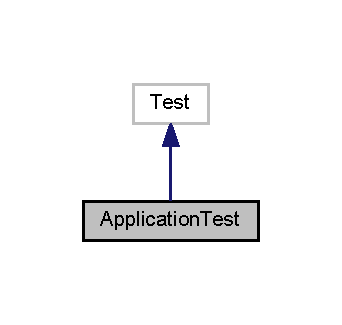
\includegraphics[width=164pt]{class_application_test__inherit__graph}
\end{center}
\end{figure}


Collaboration diagram for Application\+Test\+:\nopagebreak
\begin{figure}[H]
\begin{center}
\leavevmode
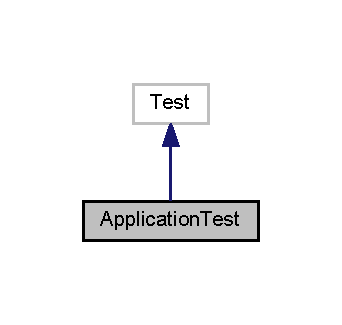
\includegraphics[width=164pt]{class_application_test__coll__graph}
\end{center}
\end{figure}
\subsection*{Protected Member Functions}
\begin{DoxyCompactItemize}
\item 
\hypertarget{class_application_test_a0ed0ce167bcb37c85c5c0bec236296d2}{}\label{class_application_test_a0ed0ce167bcb37c85c5c0bec236296d2} 
virtual void {\bfseries Set\+Up} ()
\end{DoxyCompactItemize}
\subsection*{Protected Attributes}
\begin{DoxyCompactItemize}
\item 
\hypertarget{class_application_test_ad1a2c933b0b58c4f23d7a1b51bcc30b9}{}\label{class_application_test_ad1a2c933b0b58c4f23d7a1b51bcc30b9} 
std\+::unique\+\_\+ptr$<$ \hyperlink{classae_1_1_application}{Application} $>$ {\bfseries application} = nullptr
\end{DoxyCompactItemize}


The documentation for this class was generated from the following file\+:\begin{DoxyCompactItemize}
\item 
src/application\+\_\+test.\+cc\end{DoxyCompactItemize}

\hypertarget{classae_1_1_error}{}\section{ae\+:\+:Error Class Reference}
\label{classae_1_1_error}\index{ae\+::\+Error@{ae\+::\+Error}}


Handle errors.  




{\ttfamily \#include $<$error.\+h$>$}



Inheritance diagram for ae\+:\+:Error\+:
\nopagebreak
\begin{figure}[H]
\begin{center}
\leavevmode
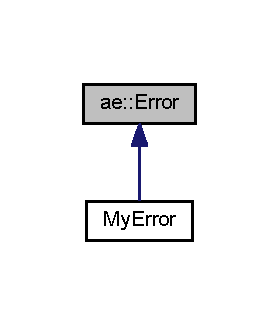
\includegraphics[width=238pt]{classae_1_1_error__inherit__graph}
\end{center}
\end{figure}


Collaboration diagram for ae\+:\+:Error\+:
\nopagebreak
\begin{figure}[H]
\begin{center}
\leavevmode
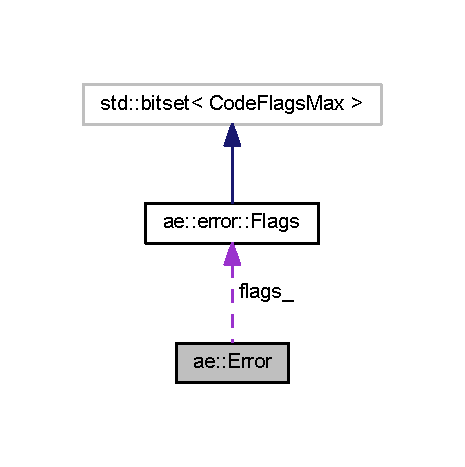
\includegraphics[width=223pt]{classae_1_1_error__coll__graph}
\end{center}
\end{figure}
\subsection*{Public Member Functions}
\begin{DoxyCompactItemize}
\item 
\hypertarget{classae_1_1_error_af8423867a7fddb42a71111b96c92c740}{}\label{classae_1_1_error_af8423867a7fddb42a71111b96c92c740} 
{\bfseries Error} (const \hyperlink{classae_1_1_error}{Error} \&)=delete
\item 
\hypertarget{classae_1_1_error_a60f2301a074178a8b3f8cf6bd37ec395}{}\label{classae_1_1_error_a60f2301a074178a8b3f8cf6bd37ec395} 
{\bfseries Error} (\hyperlink{classae_1_1_error}{Error} \&\&)=delete
\item 
\hypertarget{classae_1_1_error_a26a17a28eaed3d38349191ec5a878572}{}\label{classae_1_1_error_a26a17a28eaed3d38349191ec5a878572} 
\hyperlink{classae_1_1_error}{Error} \& {\bfseries operator=} (const \hyperlink{classae_1_1_error}{Error} \&)=delete
\item 
\hypertarget{classae_1_1_error_a5e800d8b4d0e8bccc14dd5dc815b9a08}{}\label{classae_1_1_error_a5e800d8b4d0e8bccc14dd5dc815b9a08} 
\hyperlink{classae_1_1_error}{Error} \& {\bfseries operator=} (\hyperlink{classae_1_1_error}{Error} \&\&)=delete
\item 
\hypertarget{classae_1_1_error_a5424dd175ff84fcc0dbc2bda1952b939}{}\label{classae_1_1_error_a5424dd175ff84fcc0dbc2bda1952b939} 
bool {\bfseries Is\+Success} () const noexcept
\item 
\hypertarget{classae_1_1_error_a12852602e662db19d5d7f5cc06256c46}{}\label{classae_1_1_error_a12852602e662db19d5d7f5cc06256c46} 
bool {\bfseries Is\+Error} () const noexcept
\item 
\hypertarget{classae_1_1_error_a7dbdfd03e6f6d180d1f0ded4efa10cac}{}\label{classae_1_1_error_a7dbdfd03e6f6d180d1f0ded4efa10cac} 
\hyperlink{structae_1_1error_1_1_flags}{error\+::\+Flags} {\bfseries flags} () const noexcept
\item 
virtual std\+::pair$<$ std\+::string, \hyperlink{structae_1_1error_1_1_flags}{error\+::\+Flags} $>$ \hyperlink{classae_1_1_error_ab6172fe7f6627dd726223bd4bd923693}{Diagnostic\+All} () noexcept
\begin{DoxyCompactList}\small\item\em Analyse the errors for more details. \end{DoxyCompactList}\item 
\hypertarget{classae_1_1_error_a5390c80f9eed13d8b4fce01468395187}{}\label{classae_1_1_error_a5390c80f9eed13d8b4fce01468395187} 
virtual std\+::string \hyperlink{classae_1_1_error_a5390c80f9eed13d8b4fce01468395187}{Message} () noexcept
\begin{DoxyCompactList}\small\item\em Return human-\/readble message. Alias to \hyperlink{classae_1_1_error_ab6172fe7f6627dd726223bd4bd923693}{Diagnostic\+All()}.first. \end{DoxyCompactList}\end{DoxyCompactItemize}
\subsection*{Protected Attributes}
\begin{DoxyCompactItemize}
\item 
\hyperlink{structae_1_1error_1_1_flags}{error\+::\+Flags} \hyperlink{classae_1_1_error_a323912fc2d0f697f2513d0c990478073}{flags\+\_\+}
\begin{DoxyCompactList}\small\item\em Flags state. \end{DoxyCompactList}\end{DoxyCompactItemize}


\subsection{Detailed Description}
Handle errors. 

\begin{DoxySeeAlso}{See also}
\hyperlink{structae_1_1error_1_1_flags}{ae\+::error\+::\+Flags}
\end{DoxySeeAlso}
Example \+: 
\begin{DoxyCode}
\textcolor{keyword}{class }\hyperlink{class_my_error}{MyError} : \textcolor{keyword}{public} \hyperlink{classae_1_1_error}{ae::Error} \{
    \hyperlink{class_my_error}{MyError}(\textcolor{keywordtype}{int} code);
    \textcolor{keyword}{virtual} \hyperlink{class_my_error}{MyError}();
\}

MyError::MyError(\textcolor{keywordtype}{int} code) \{
    \textcolor{keywordflow}{if}(code < 0)
        \hyperlink{classae_1_1_error_a323912fc2d0f697f2513d0c990478073}{flags\_}.set\_error();
\}

\textcolor{keywordtype}{int} main() \{
    \hyperlink{class_my_error}{MyError} error(-1);

    \textcolor{keywordflow}{if} (error.IsError) \textcolor{keywordflow}{throw} error.Message();
\}
\end{DoxyCode}
 

\subsection{Member Function Documentation}
\hypertarget{classae_1_1_error_ab6172fe7f6627dd726223bd4bd923693}{}\label{classae_1_1_error_ab6172fe7f6627dd726223bd4bd923693} 
\index{ae\+::\+Error@{ae\+::\+Error}!Diagnostic\+All@{Diagnostic\+All}}
\index{Diagnostic\+All@{Diagnostic\+All}!ae\+::\+Error@{ae\+::\+Error}}
\subsubsection{\texorpdfstring{Diagnostic\+All()}{DiagnosticAll()}}
{\footnotesize\ttfamily std\+::pair$<$ std\+::string, \hyperlink{structae_1_1error_1_1_flags}{error\+::\+Flags} $>$ ae\+::\+Error\+::\+Diagnostic\+All (\begin{DoxyParamCaption}{ }\end{DoxyParamCaption})\hspace{0.3cm}{\ttfamily [virtual]}, {\ttfamily [noexcept]}}



Analyse the errors for more details. 

\begin{DoxyReturn}{Returns}
a The first element is for humans and the second is for the program.
\end{DoxyReturn}
Example \+:


\begin{DoxyCode}
\textcolor{keyword}{auto} diagnostic = \hyperlink{class_my_error}{MyError}(); \textcolor{comment}{// See ae::Error}
\textcolor{keywordflow}{if}(diagnostic.second.is\_error())
\textcolor{keywordflow}{throw} diagnostics.first
\end{DoxyCode}
 

Reimplemented in \hyperlink{classae_1_1error_1_1_vulkan_a1446494fd8ab1b5fc4b9ca8c27b37e8a}{ae\+::error\+::\+Vulkan}.



\subsection{Member Data Documentation}
\hypertarget{classae_1_1_error_a323912fc2d0f697f2513d0c990478073}{}\label{classae_1_1_error_a323912fc2d0f697f2513d0c990478073} 
\index{ae\+::\+Error@{ae\+::\+Error}!flags\+\_\+@{flags\+\_\+}}
\index{flags\+\_\+@{flags\+\_\+}!ae\+::\+Error@{ae\+::\+Error}}
\subsubsection{\texorpdfstring{flags\+\_\+}{flags\_}}
{\footnotesize\ttfamily \hyperlink{structae_1_1error_1_1_flags}{error\+::\+Flags} ae\+::\+Error\+::flags\+\_\+\hspace{0.3cm}{\ttfamily [protected]}}



Flags state. 

\begin{DoxySeeAlso}{See also}
\hyperlink{structae_1_1error_1_1_flags}{ae\+::error\+::\+Flags} 
\end{DoxySeeAlso}


The documentation for this class was generated from the following files\+:\begin{DoxyCompactItemize}
\item 
src/error.\+h\item 
src/error.\+cc\end{DoxyCompactItemize}

\hypertarget{class_error_flags_test}{}\section{Error\+Flags\+Test Class Reference}
\label{class_error_flags_test}\index{Error\+Flags\+Test@{Error\+Flags\+Test}}


The fixture for testing class error\+::\+Flags.  




Inheritance diagram for Error\+Flags\+Test\+:
\nopagebreak
\begin{figure}[H]
\begin{center}
\leavevmode
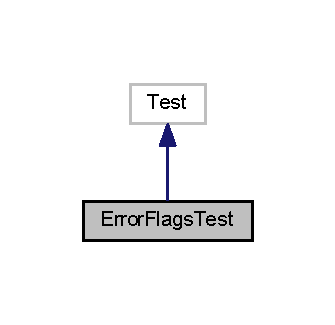
\includegraphics[width=161pt]{class_error_flags_test__inherit__graph}
\end{center}
\end{figure}


Collaboration diagram for Error\+Flags\+Test\+:
\nopagebreak
\begin{figure}[H]
\begin{center}
\leavevmode
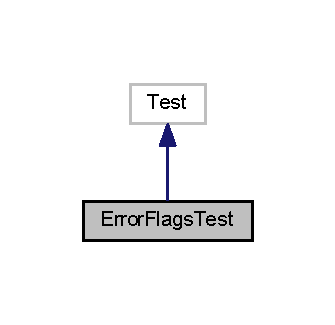
\includegraphics[width=161pt]{class_error_flags_test__coll__graph}
\end{center}
\end{figure}
\subsection*{Protected Member Functions}
\begin{DoxyCompactItemize}
\item 
\hypertarget{class_error_flags_test_a14e4a93a156e1cb9e96b26d2a1dae27f}{}\label{class_error_flags_test_a14e4a93a156e1cb9e96b26d2a1dae27f} 
virtual void \hyperlink{class_error_flags_test_a14e4a93a156e1cb9e96b26d2a1dae27f}{Set\+Up} ()
\begin{DoxyCompactList}\small\item\em Set fixture. \end{DoxyCompactList}\end{DoxyCompactItemize}
\subsection*{Protected Attributes}
\begin{DoxyCompactItemize}
\item 
\hypertarget{class_error_flags_test_ad93619dfba84c24ed82eee5724e769ef}{}\label{class_error_flags_test_ad93619dfba84c24ed82eee5724e769ef} 
std\+::unique\+\_\+ptr$<$ \hyperlink{structae_1_1error_1_1_flags}{error\+::\+Flags} $>$ \hyperlink{class_error_flags_test_ad93619dfba84c24ed82eee5724e769ef}{diagnostic} = nullptr
\begin{DoxyCompactList}\small\item\em Pointer to an instance class test. \end{DoxyCompactList}\end{DoxyCompactItemize}


\subsection{Detailed Description}
The fixture for testing class error\+::\+Flags. 

The documentation for this class was generated from the following file\+:\begin{DoxyCompactItemize}
\item 
src/error/flags\+\_\+test.\+cc\end{DoxyCompactItemize}

\hypertarget{class_error_test}{}\section{Error\+Test Class Reference}
\label{class_error_test}\index{Error\+Test@{Error\+Test}}


Inheritance diagram for Error\+Test\+:\nopagebreak
\begin{figure}[H]
\begin{center}
\leavevmode
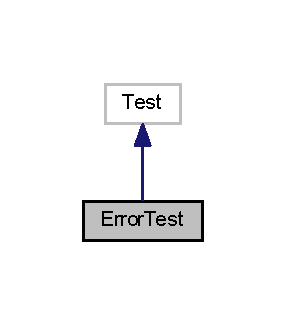
\includegraphics[width=137pt]{class_error_test__inherit__graph}
\end{center}
\end{figure}


Collaboration diagram for Error\+Test\+:\nopagebreak
\begin{figure}[H]
\begin{center}
\leavevmode
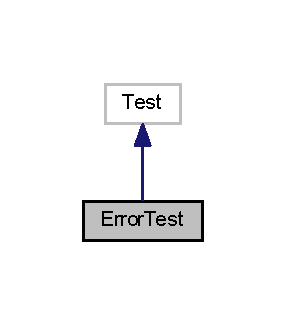
\includegraphics[width=137pt]{class_error_test__coll__graph}
\end{center}
\end{figure}
\subsection*{Protected Member Functions}
\begin{DoxyCompactItemize}
\item 
\hypertarget{class_error_test_a282955d762cb937af68efea62c37fccd}{}\label{class_error_test_a282955d762cb937af68efea62c37fccd} 
virtual void {\bfseries Set\+Up} ()
\end{DoxyCompactItemize}
\subsection*{Protected Attributes}
\begin{DoxyCompactItemize}
\item 
\hypertarget{class_error_test_a0f59553359b5a5fc50771e391478c1f4}{}\label{class_error_test_a0f59553359b5a5fc50771e391478c1f4} 
std\+::unique\+\_\+ptr$<$ \hyperlink{class_my_error}{My\+Error} $>$ {\bfseries error\+\_\+success} = nullptr
\item 
\hypertarget{class_error_test_a3f26eee630d733a24b1b192453abdc36}{}\label{class_error_test_a3f26eee630d733a24b1b192453abdc36} 
std\+::unique\+\_\+ptr$<$ \hyperlink{class_my_error}{My\+Error} $>$ {\bfseries error\+\_\+error} = nullptr
\end{DoxyCompactItemize}


The documentation for this class was generated from the following file\+:\begin{DoxyCompactItemize}
\item 
src/error\+\_\+test.\+cc\end{DoxyCompactItemize}

\hypertarget{class_error_vulkan_test}{}\section{Error\+Vulkan\+Test Class Reference}
\label{class_error_vulkan_test}\index{Error\+Vulkan\+Test@{Error\+Vulkan\+Test}}


The fixture for testing class error\+::\+Vulkan.  




Inheritance diagram for Error\+Vulkan\+Test\+:
\nopagebreak
\begin{figure}[H]
\begin{center}
\leavevmode
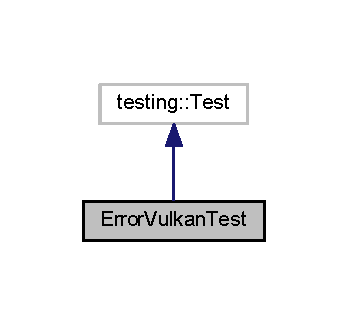
\includegraphics[width=167pt]{class_error_vulkan_test__inherit__graph}
\end{center}
\end{figure}


Collaboration diagram for Error\+Vulkan\+Test\+:
\nopagebreak
\begin{figure}[H]
\begin{center}
\leavevmode
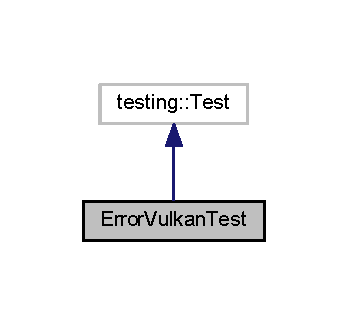
\includegraphics[width=167pt]{class_error_vulkan_test__coll__graph}
\end{center}
\end{figure}
\subsection*{Protected Member Functions}
\begin{DoxyCompactItemize}
\item 
\hypertarget{class_error_vulkan_test_a5ae9d99b5e62289e47e4e7af7ab334ab}{}\label{class_error_vulkan_test_a5ae9d99b5e62289e47e4e7af7ab334ab} 
virtual void \hyperlink{class_error_vulkan_test_a5ae9d99b5e62289e47e4e7af7ab334ab}{Set\+Up} ()
\begin{DoxyCompactList}\small\item\em Set fixture. \end{DoxyCompactList}\end{DoxyCompactItemize}
\subsection*{Protected Attributes}
\begin{DoxyCompactItemize}
\item 
\hypertarget{class_error_vulkan_test_a2413e0ba8b4ef1f1d872554142f24fab}{}\label{class_error_vulkan_test_a2413e0ba8b4ef1f1d872554142f24fab} 
std\+::unique\+\_\+ptr$<$ error\+::\+Vulkan $>$ \hyperlink{class_error_vulkan_test_a2413e0ba8b4ef1f1d872554142f24fab}{vulkan\+\_\+error} = nullptr
\begin{DoxyCompactList}\small\item\em Pointer to an instance class test. \end{DoxyCompactList}\end{DoxyCompactItemize}


\subsection{Detailed Description}
The fixture for testing class error\+::\+Vulkan. 

The documentation for this class was generated from the following file\+:\begin{DoxyCompactItemize}
\item 
src/error/vulkan\+\_\+test.\+cc\end{DoxyCompactItemize}

\hypertarget{structae_1_1error_1_1_flags}{}\section{ae\+:\+:error\+:\+:Flags Struct Reference}
\label{structae_1_1error_1_1_flags}\index{ae\+::error\+::\+Flags@{ae\+::error\+::\+Flags}}


Bit state flags of the error.  




{\ttfamily \#include $<$flags.\+h$>$}



Inheritance diagram for ae\+:\+:error\+:\+:Flags\+:
\nopagebreak
\begin{figure}[H]
\begin{center}
\leavevmode
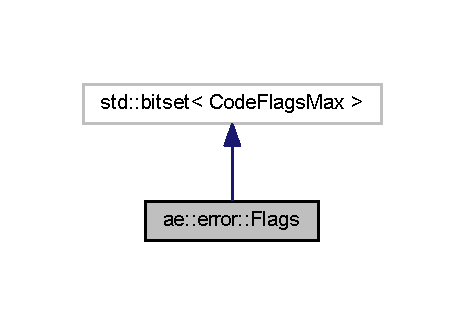
\includegraphics[width=223pt]{structae_1_1error_1_1_flags__inherit__graph}
\end{center}
\end{figure}


Collaboration diagram for ae\+:\+:error\+:\+:Flags\+:
\nopagebreak
\begin{figure}[H]
\begin{center}
\leavevmode
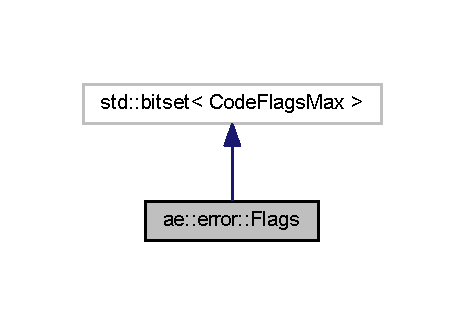
\includegraphics[width=223pt]{structae_1_1error_1_1_flags__coll__graph}
\end{center}
\end{figure}
\subsection*{Public Types}
\begin{DoxyCompactItemize}
\item 
\hypertarget{structae_1_1error_1_1_flags_ac202ad39c23bb50a535c1a9af3a8c0b1}{}\label{structae_1_1error_1_1_flags_ac202ad39c23bb50a535c1a9af3a8c0b1} 
enum \hyperlink{structae_1_1error_1_1_flags_ac202ad39c23bb50a535c1a9af3a8c0b1}{Code} \{ {\bfseries k\+Success} = 0, 
{\bfseries k\+Verbose} = 1
 \}\begin{DoxyCompactList}\small\item\em Bits positions in \hyperlink{structae_1_1error_1_1_flags}{ae\+::error\+::\+Flags}. \end{DoxyCompactList}
\item 
\hypertarget{structae_1_1error_1_1_flags_a9a0599e8c956ab8b269a83e68706aff4}{}\label{structae_1_1error_1_1_flags_a9a0599e8c956ab8b269a83e68706aff4} 
using \hyperlink{structae_1_1error_1_1_flags_a9a0599e8c956ab8b269a83e68706aff4}{base} = std\+::bitset$<$ Code\+Flags\+Max $>$
\begin{DoxyCompactList}\small\item\em Base class of \hyperlink{structae_1_1error_1_1_flags}{ae\+::error\+::\+Flags}. \end{DoxyCompactList}\end{DoxyCompactItemize}
\subsection*{Public Member Functions}
\begin{DoxyCompactItemize}
\item 
\hypertarget{structae_1_1error_1_1_flags_adbb5b192eaf777f86ca7ba817579d06b}{}\label{structae_1_1error_1_1_flags_adbb5b192eaf777f86ca7ba817579d06b} 
void \hyperlink{structae_1_1error_1_1_flags_adbb5b192eaf777f86ca7ba817579d06b}{Set\+Success} () noexcept
\begin{DoxyCompactList}\small\item\em Set the k\+Success bit flag to true. \end{DoxyCompactList}\item 
\hypertarget{structae_1_1error_1_1_flags_a71313318889dccdaf15ab4956afefbaf}{}\label{structae_1_1error_1_1_flags_a71313318889dccdaf15ab4956afefbaf} 
void \hyperlink{structae_1_1error_1_1_flags_a71313318889dccdaf15ab4956afefbaf}{Reset\+Success} () noexcept
\begin{DoxyCompactList}\small\item\em Set the k\+Success bit flag to false. \end{DoxyCompactList}\item 
\hypertarget{structae_1_1error_1_1_flags_a7c28232700cf13cef02bb0ba4c6db15b}{}\label{structae_1_1error_1_1_flags_a7c28232700cf13cef02bb0ba4c6db15b} 
bool \hyperlink{structae_1_1error_1_1_flags_a7c28232700cf13cef02bb0ba4c6db15b}{Is\+Success} () const noexcept
\begin{DoxyCompactList}\small\item\em Returns the k\+Success bit flag. \end{DoxyCompactList}\item 
\hypertarget{structae_1_1error_1_1_flags_a0564df5fa77cd2ef1dd7dcb0ce4105b9}{}\label{structae_1_1error_1_1_flags_a0564df5fa77cd2ef1dd7dcb0ce4105b9} 
void \hyperlink{structae_1_1error_1_1_flags_a0564df5fa77cd2ef1dd7dcb0ce4105b9}{Set\+Error} () noexcept
\begin{DoxyCompactList}\small\item\em Alias to \hyperlink{structae_1_1error_1_1_flags_a71313318889dccdaf15ab4956afefbaf}{Reset\+Success()}. \end{DoxyCompactList}\item 
\hypertarget{structae_1_1error_1_1_flags_a9b13f39f7bbead91006bc776d32cb14e}{}\label{structae_1_1error_1_1_flags_a9b13f39f7bbead91006bc776d32cb14e} 
void \hyperlink{structae_1_1error_1_1_flags_a9b13f39f7bbead91006bc776d32cb14e}{Reset\+Error} () noexcept
\begin{DoxyCompactList}\small\item\em Alias to \hyperlink{structae_1_1error_1_1_flags_adbb5b192eaf777f86ca7ba817579d06b}{Set\+Success()}. \end{DoxyCompactList}\item 
\hypertarget{structae_1_1error_1_1_flags_af9751a6f34f4a83bbe402d97e9af646d}{}\label{structae_1_1error_1_1_flags_af9751a6f34f4a83bbe402d97e9af646d} 
bool \hyperlink{structae_1_1error_1_1_flags_af9751a6f34f4a83bbe402d97e9af646d}{Is\+Error} () const noexcept
\begin{DoxyCompactList}\small\item\em Invert \hyperlink{structae_1_1error_1_1_flags_a7c28232700cf13cef02bb0ba4c6db15b}{Is\+Success()}. \end{DoxyCompactList}\item 
\hypertarget{structae_1_1error_1_1_flags_aa80a0e830d0f0a390c5c8158b909fc29}{}\label{structae_1_1error_1_1_flags_aa80a0e830d0f0a390c5c8158b909fc29} 
void \hyperlink{structae_1_1error_1_1_flags_aa80a0e830d0f0a390c5c8158b909fc29}{Set\+Verbose} () noexcept
\begin{DoxyCompactList}\small\item\em Set the k\+Verbose bit flag to true. \end{DoxyCompactList}\item 
\hypertarget{structae_1_1error_1_1_flags_a32b80335f90ce234cf1d1d172e3c30a5}{}\label{structae_1_1error_1_1_flags_a32b80335f90ce234cf1d1d172e3c30a5} 
void \hyperlink{structae_1_1error_1_1_flags_a32b80335f90ce234cf1d1d172e3c30a5}{Reset\+Verbose} () noexcept
\begin{DoxyCompactList}\small\item\em Set the k\+Verbose bit flag to false. \end{DoxyCompactList}\item 
\hypertarget{structae_1_1error_1_1_flags_ab47c8ae55803bbca67c8328ca2ca44bc}{}\label{structae_1_1error_1_1_flags_ab47c8ae55803bbca67c8328ca2ca44bc} 
bool \hyperlink{structae_1_1error_1_1_flags_ab47c8ae55803bbca67c8328ca2ca44bc}{Is\+Verbose} () const noexcept
\begin{DoxyCompactList}\small\item\em Returns the k\+Verbose bit flag. \end{DoxyCompactList}\end{DoxyCompactItemize}
{\bf }\par
\begin{DoxyCompactItemize}
\item 
\hypertarget{structae_1_1error_1_1_flags_a20c944aed64eceeec6e4eb34553f499e}{}\label{structae_1_1error_1_1_flags_a20c944aed64eceeec6e4eb34553f499e} 
{\bfseries Flags} (const \hyperlink{structae_1_1error_1_1_flags}{Flags} \&)
\item 
\hypertarget{structae_1_1error_1_1_flags_a02aa5d86c37d9f80a4de795fb81b1c19}{}\label{structae_1_1error_1_1_flags_a02aa5d86c37d9f80a4de795fb81b1c19} 
{\bfseries Flags} (\hyperlink{structae_1_1error_1_1_flags}{Flags} \&\&)
\item 
\hypertarget{structae_1_1error_1_1_flags_a0a215694736b3b865b639c5b5abd173c}{}\label{structae_1_1error_1_1_flags_a0a215694736b3b865b639c5b5abd173c} 
\hyperlink{structae_1_1error_1_1_flags}{Flags} \& {\bfseries operator=} (const \hyperlink{structae_1_1error_1_1_flags}{Flags} \&)
\item 
\hypertarget{structae_1_1error_1_1_flags_ae08dbfd93ce5d40516fc3b27fb82d196}{}\label{structae_1_1error_1_1_flags_ae08dbfd93ce5d40516fc3b27fb82d196} 
\hyperlink{structae_1_1error_1_1_flags}{Flags} \& {\bfseries operator=} (\hyperlink{structae_1_1error_1_1_flags}{Flags} \&\&)
\end{DoxyCompactItemize}



\subsection{Detailed Description}
Bit state flags of the error. 

Example \+:


\begin{DoxyCode}
\hyperlink{structae_1_1error_1_1_flags}{ae::error::Flags} flags;
\textcolor{keywordflow}{if}(random\_number % 2)
    flags.\hyperlink{structae_1_1error_1_1_flags_a0564df5fa77cd2ef1dd7dcb0ce4105b9}{SetError}();
\end{DoxyCode}
 

The documentation for this struct was generated from the following files\+:\begin{DoxyCompactItemize}
\item 
src/error/flags.\+h\item 
src/error/flags.\+cc\end{DoxyCompactItemize}

\hypertarget{classae_1_1_g_l_f_w}{}\section{ae\+:\+:G\+L\+FW Class Reference}
\label{classae_1_1_g_l_f_w}\index{ae\+::\+G\+L\+FW@{ae\+::\+G\+L\+FW}}


Inheritance diagram for ae\+:\+:G\+L\+FW\+:
\nopagebreak
\begin{figure}[H]
\begin{center}
\leavevmode
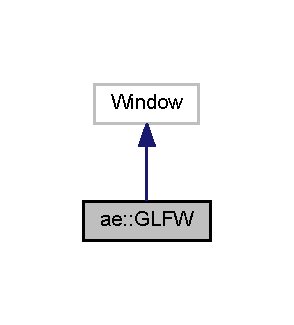
\includegraphics[width=147pt]{classae_1_1_g_l_f_w__inherit__graph}
\end{center}
\end{figure}


Collaboration diagram for ae\+:\+:G\+L\+FW\+:
\nopagebreak
\begin{figure}[H]
\begin{center}
\leavevmode
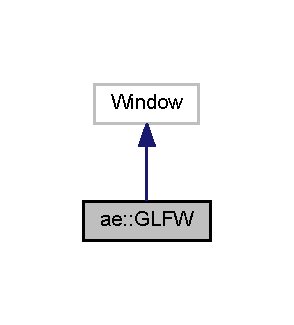
\includegraphics[width=147pt]{classae_1_1_g_l_f_w__coll__graph}
\end{center}
\end{figure}
\subsection*{Public Member Functions}
\begin{DoxyCompactItemize}
\item 
\hypertarget{classae_1_1_g_l_f_w_a3f91f115acec8b4abc62d5f3f51c8674}{}\label{classae_1_1_g_l_f_w_a3f91f115acec8b4abc62d5f3f51c8674} 
{\bfseries G\+L\+FW} (const \hyperlink{classae_1_1_g_l_f_w}{G\+L\+FW} \&)=delete
\item 
\hypertarget{classae_1_1_g_l_f_w_afaa7b320295e3437529407c51d279e31}{}\label{classae_1_1_g_l_f_w_afaa7b320295e3437529407c51d279e31} 
\hyperlink{classae_1_1_g_l_f_w}{G\+L\+FW} \& {\bfseries operator=} (const \hyperlink{classae_1_1_g_l_f_w}{G\+L\+FW} \&)=delete
\item 
\hypertarget{classae_1_1_g_l_f_w_af3d2c2732b89aefc5596c0ec44d39b9e}{}\label{classae_1_1_g_l_f_w_af3d2c2732b89aefc5596c0ec44d39b9e} 
\hyperlink{classae_1_1_g_l_f_w}{G\+L\+FW} \& {\bfseries operator=} (\hyperlink{classae_1_1_g_l_f_w}{G\+L\+FW} \&\&)=default
\item 
\hypertarget{classae_1_1_g_l_f_w_a968689c66e954617a81704025c73f016}{}\label{classae_1_1_g_l_f_w_a968689c66e954617a81704025c73f016} 
{\bfseries G\+L\+FW} (\hyperlink{classae_1_1_g_l_f_w}{G\+L\+FW} \&\&)
\item 
\hypertarget{classae_1_1_g_l_f_w_a3df047bd36e3e64d79e99038762b5ce2}{}\label{classae_1_1_g_l_f_w_a3df047bd36e3e64d79e99038762b5ce2} 
bool {\bfseries Pool\+Event} () noexcept override
\item 
\hypertarget{classae_1_1_g_l_f_w_a5ec4f5b56e7f9a2011aaa4716503c563}{}\label{classae_1_1_g_l_f_w_a5ec4f5b56e7f9a2011aaa4716503c563} 
std\+::vector$<$ const char $\ast$ $>$ {\bfseries extensions} () const noexcept override
\end{DoxyCompactItemize}
\subsection*{Additional Inherited Members}


The documentation for this class was generated from the following files\+:\begin{DoxyCompactItemize}
\item 
src/window/glfw.\+h\item 
src/window/glfw.\+cc\end{DoxyCompactItemize}

\hypertarget{classae_1_1_instance}{}\section{ae\+:\+:Instance Class Reference}
\label{classae_1_1_instance}\index{ae\+::\+Instance@{ae\+::\+Instance}}
\subsection*{Public Member Functions}
\begin{DoxyCompactItemize}
\item 
\hypertarget{classae_1_1_instance_a48d480419ea5ee601db2bacf7b6d48d2}{}\label{classae_1_1_instance_a48d480419ea5ee601db2bacf7b6d48d2} 
{\bfseries Instance} (const \hyperlink{classae_1_1_instance}{Instance} \&)
\item 
\hypertarget{classae_1_1_instance_ac0b8b262e4aa1e2ff3eb0e8839f9868c}{}\label{classae_1_1_instance_ac0b8b262e4aa1e2ff3eb0e8839f9868c} 
{\bfseries Instance} (\hyperlink{classae_1_1_instance}{Instance} \&\&)
\item 
\hypertarget{classae_1_1_instance_ad01e1dd78cb36b0a112770281a836f19}{}\label{classae_1_1_instance_ad01e1dd78cb36b0a112770281a836f19} 
\hyperlink{classae_1_1_instance}{Instance} \& {\bfseries operator=} (const \hyperlink{classae_1_1_instance}{Instance} \&)
\item 
\hypertarget{classae_1_1_instance_a2d73116829ee705a15c32f9e7c113524}{}\label{classae_1_1_instance_a2d73116829ee705a15c32f9e7c113524} 
\hyperlink{classae_1_1_instance}{Instance} \& {\bfseries operator=} (\hyperlink{classae_1_1_instance}{Instance} \&\&)
\item 
\hypertarget{classae_1_1_instance_a9de8fa013e11a71aa6e09f142aa1a927}{}\label{classae_1_1_instance_a9de8fa013e11a71aa6e09f142aa1a927} 
Vk\+Result {\bfseries Create} () noexcept
\item 
\hypertarget{classae_1_1_instance_a0aaff634cda5a58a37ae93b2f577721d}{}\label{classae_1_1_instance_a0aaff634cda5a58a37ae93b2f577721d} 
std\+::vector$<$ const char $\ast$ $>$ {\bfseries extensions} () const noexcept
\item 
\hypertarget{classae_1_1_instance_a880ed1eaf9b821ac616865821a5f15ef}{}\label{classae_1_1_instance_a880ed1eaf9b821ac616865821a5f15ef} 
void {\bfseries Add\+Extensions} (const std\+::vector$<$ const char $\ast$$>$ \&) noexcept
\item 
\hypertarget{classae_1_1_instance_a1546a926e92a106a3829ce6b8729de42}{}\label{classae_1_1_instance_a1546a926e92a106a3829ce6b8729de42} 
std\+::vector$<$ Vk\+Extension\+Properties $>$ {\bfseries Available\+Extensions} () const noexcept
\item 
\hypertarget{classae_1_1_instance_a135806a6a6de15f61b3a66c20aa1c738}{}\label{classae_1_1_instance_a135806a6a6de15f61b3a66c20aa1c738} 
std\+::vector$<$ const char $\ast$ $>$ {\bfseries Available\+Extensions\+Name} () const noexcept
\item 
\hypertarget{classae_1_1_instance_a50d9c6f77415412fc5cedc2838abc527}{}\label{classae_1_1_instance_a50d9c6f77415412fc5cedc2838abc527} 
std\+::vector$<$ const char $\ast$ $>$ {\bfseries Missing\+Extensions} () const noexcept
\item 
\hypertarget{classae_1_1_instance_a356579044ea77c9cc14723f0b7d7a52d}{}\label{classae_1_1_instance_a356579044ea77c9cc14723f0b7d7a52d} 
std\+::vector$<$ const char $\ast$ $>$ {\bfseries validations} () const noexcept
\item 
\hypertarget{classae_1_1_instance_ae00908ee44223a209184015514a35685}{}\label{classae_1_1_instance_ae00908ee44223a209184015514a35685} 
void {\bfseries Add\+Validations} (const std\+::vector$<$ const char $\ast$$>$ \&) noexcept
\item 
\hypertarget{classae_1_1_instance_ae6ab8f05e13a1efeb8bcc4a6972b9072}{}\label{classae_1_1_instance_ae6ab8f05e13a1efeb8bcc4a6972b9072} 
void {\bfseries Add\+Default\+Validations} () noexcept
\item 
\hypertarget{classae_1_1_instance_a6b46129d8c0b5d204eab1a1cecb5b221}{}\label{classae_1_1_instance_a6b46129d8c0b5d204eab1a1cecb5b221} 
std\+::vector$<$ Vk\+Layer\+Properties $>$ {\bfseries Available\+Validations} () const noexcept
\item 
\hypertarget{classae_1_1_instance_a3439df7740449cf58fe3613c957b359f}{}\label{classae_1_1_instance_a3439df7740449cf58fe3613c957b359f} 
std\+::vector$<$ const char $\ast$ $>$ {\bfseries Available\+Validations\+Name} () const noexcept
\item 
\hypertarget{classae_1_1_instance_aa76edbae91362fadb47c743b6f4298be}{}\label{classae_1_1_instance_aa76edbae91362fadb47c743b6f4298be} 
std\+::vector$<$ const char $\ast$ $>$ {\bfseries Missing\+Validations} () const noexcept
\end{DoxyCompactItemize}
\subsection*{Public Attributes}
\begin{DoxyCompactItemize}
\item 
const std\+::vector$<$ const char $\ast$ $>$ {\bfseries k\+Default\+Validations}
\item 
\hypertarget{classae_1_1_instance_a5dabba3cfc37e4f41a5c8a0b710f2adf}{}\label{classae_1_1_instance_a5dabba3cfc37e4f41a5c8a0b710f2adf} 
bool {\bfseries enable\+\_\+default\+\_\+validations} = true
\end{DoxyCompactItemize}


\subsection{Member Data Documentation}
\hypertarget{classae_1_1_instance_a51fa0c0f46de73754c52841fc458d4ac}{}\label{classae_1_1_instance_a51fa0c0f46de73754c52841fc458d4ac} 
\index{ae\+::\+Instance@{ae\+::\+Instance}!k\+Default\+Validations@{k\+Default\+Validations}}
\index{k\+Default\+Validations@{k\+Default\+Validations}!ae\+::\+Instance@{ae\+::\+Instance}}
\subsubsection{\texorpdfstring{k\+Default\+Validations}{kDefaultValidations}}
{\footnotesize\ttfamily const std\+::vector$<$const char $\ast$$>$ ae\+::\+Instance\+::k\+Default\+Validations}

{\bfseries Initial value\+:}
\begin{DoxyCode}
= \{
        \textcolor{stringliteral}{"VK\_LAYER\_LUNARG\_standard\_validation"}\}
\end{DoxyCode}


The documentation for this class was generated from the following files\+:\begin{DoxyCompactItemize}
\item 
src/instance.\+h\item 
src/instance.\+cc\end{DoxyCompactItemize}

\hypertarget{class_instance_test}{}\section{Instance\+Test Class Reference}
\label{class_instance_test}\index{Instance\+Test@{Instance\+Test}}


Inheritance diagram for Instance\+Test\+:\nopagebreak
\begin{figure}[H]
\begin{center}
\leavevmode
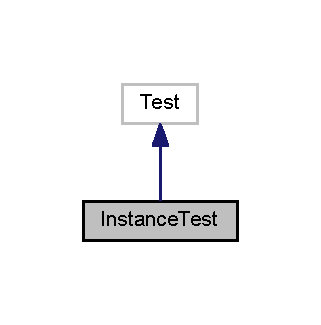
\includegraphics[width=154pt]{class_instance_test__inherit__graph}
\end{center}
\end{figure}


Collaboration diagram for Instance\+Test\+:\nopagebreak
\begin{figure}[H]
\begin{center}
\leavevmode
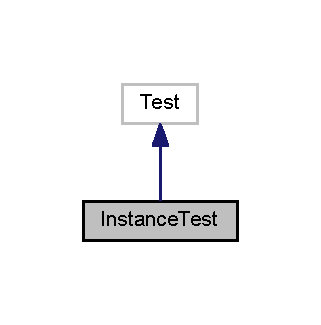
\includegraphics[width=154pt]{class_instance_test__coll__graph}
\end{center}
\end{figure}
\subsection*{Protected Member Functions}
\begin{DoxyCompactItemize}
\item 
\hypertarget{class_instance_test_aada9591781662307abc3e7511d14187c}{}\label{class_instance_test_aada9591781662307abc3e7511d14187c} 
virtual void {\bfseries Set\+Up} ()
\end{DoxyCompactItemize}
\subsection*{Protected Attributes}
\begin{DoxyCompactItemize}
\item 
\hypertarget{class_instance_test_ae818f7a311cce549e005cd651a5e4ff1}{}\label{class_instance_test_ae818f7a311cce549e005cd651a5e4ff1} 
std\+::unique\+\_\+ptr$<$ \hyperlink{classae_1_1_instance}{Instance} $>$ {\bfseries instance} = nullptr
\end{DoxyCompactItemize}


The documentation for this class was generated from the following file\+:\begin{DoxyCompactItemize}
\item 
src/instance\+\_\+test.\+cc\end{DoxyCompactItemize}

\hypertarget{class_my_error}{}\section{My\+Error Class Reference}
\label{class_my_error}\index{My\+Error@{My\+Error}}


Inheritance diagram for My\+Error\+:\nopagebreak
\begin{figure}[H]
\begin{center}
\leavevmode
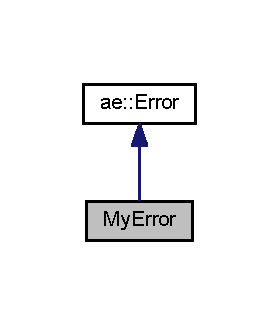
\includegraphics[width=134pt]{class_my_error__inherit__graph}
\end{center}
\end{figure}


Collaboration diagram for My\+Error\+:\nopagebreak
\begin{figure}[H]
\begin{center}
\leavevmode
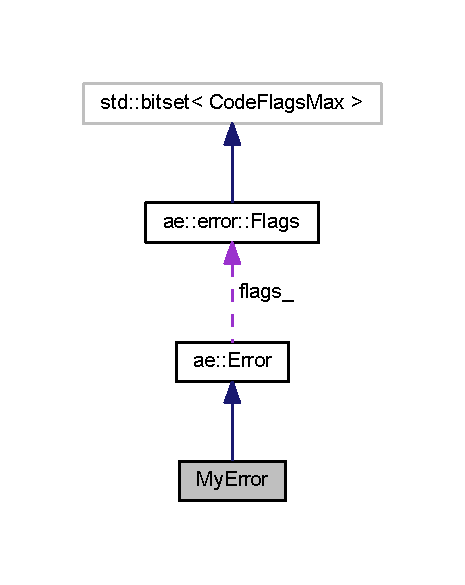
\includegraphics[width=223pt]{class_my_error__coll__graph}
\end{center}
\end{figure}
\subsection*{Public Member Functions}
\begin{DoxyCompactItemize}
\item 
\hypertarget{class_my_error_a92df252c67b7a3589f8aba5e7f197eba}{}\label{class_my_error_a92df252c67b7a3589f8aba5e7f197eba} 
{\bfseries My\+Error} (int code)
\end{DoxyCompactItemize}
\subsection*{Additional Inherited Members}


The documentation for this class was generated from the following file\+:\begin{DoxyCompactItemize}
\item 
src/error\+\_\+test.\+cc\end{DoxyCompactItemize}

\hypertarget{classae_1_1_singleton}{}\section{ae\+:\+:Singleton$<$ T $>$ Class Template Reference}
\label{classae_1_1_singleton}\index{ae\+::\+Singleton$<$ T $>$@{ae\+::\+Singleton$<$ T $>$}}


Inheritance diagram for ae\+:\+:Singleton$<$ T $>$\+:
\nopagebreak
\begin{figure}[H]
\begin{center}
\leavevmode
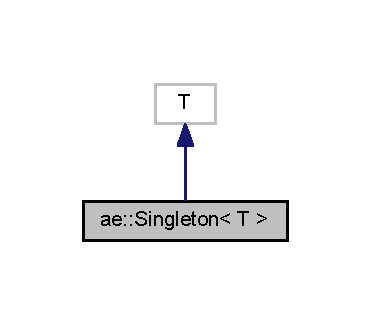
\includegraphics[width=178pt]{classae_1_1_singleton__inherit__graph}
\end{center}
\end{figure}


Collaboration diagram for ae\+:\+:Singleton$<$ T $>$\+:
\nopagebreak
\begin{figure}[H]
\begin{center}
\leavevmode
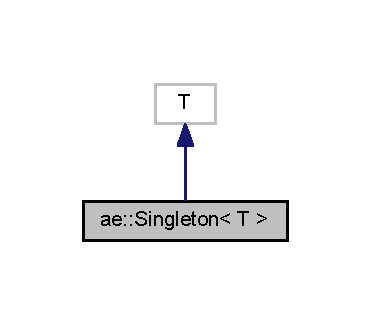
\includegraphics[width=178pt]{classae_1_1_singleton__coll__graph}
\end{center}
\end{figure}
\subsection*{Static Public Member Functions}
\begin{DoxyCompactItemize}
\item 
\hypertarget{classae_1_1_singleton_abc6b9a3fe47623032128dd1963db9a7b}{}\label{classae_1_1_singleton_abc6b9a3fe47623032128dd1963db9a7b} 
static std\+::shared\+\_\+ptr$<$ T $>$ {\bfseries create} (bool reset=false)
\end{DoxyCompactItemize}


The documentation for this class was generated from the following file\+:\begin{DoxyCompactItemize}
\item 
src/singleton.\+h\end{DoxyCompactItemize}

\hypertarget{classae_1_1error_1_1_vulkan}{}\section{ae\+:\+:error\+:\+:Vulkan Class Reference}
\label{classae_1_1error_1_1_vulkan}\index{ae\+::error\+::\+Vulkan@{ae\+::error\+::\+Vulkan}}


Inheritance diagram for ae\+:\+:error\+:\+:Vulkan\+:\nopagebreak
\begin{figure}[H]
\begin{center}
\leavevmode
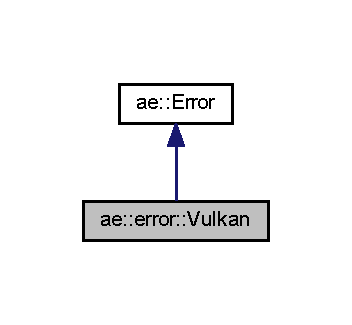
\includegraphics[width=169pt]{classae_1_1error_1_1_vulkan__inherit__graph}
\end{center}
\end{figure}


Collaboration diagram for ae\+:\+:error\+:\+:Vulkan\+:\nopagebreak
\begin{figure}[H]
\begin{center}
\leavevmode
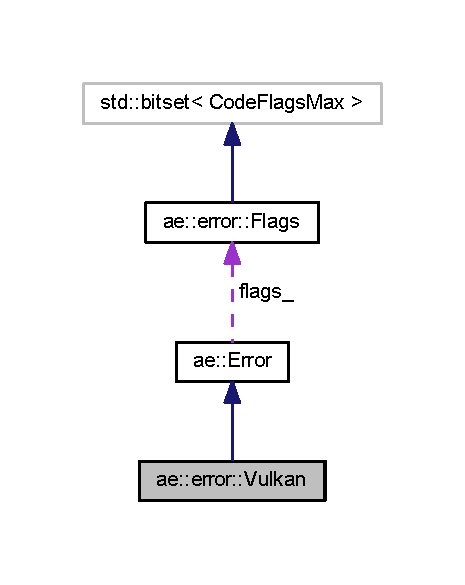
\includegraphics[width=223pt]{classae_1_1error_1_1_vulkan__coll__graph}
\end{center}
\end{figure}
\subsection*{Public Member Functions}
\begin{DoxyCompactItemize}
\item 
\hypertarget{classae_1_1error_1_1_vulkan_aa5a9db1b119cdba0e3833045764b8bc4}{}\label{classae_1_1error_1_1_vulkan_aa5a9db1b119cdba0e3833045764b8bc4} 
{\bfseries Vulkan} (const \hyperlink{classae_1_1error_1_1_vulkan}{Vulkan} \&)
\item 
\hypertarget{classae_1_1error_1_1_vulkan_a3b5c68df25fbe1acd003045560e2bb70}{}\label{classae_1_1error_1_1_vulkan_a3b5c68df25fbe1acd003045560e2bb70} 
{\bfseries Vulkan} (\hyperlink{classae_1_1error_1_1_vulkan}{Vulkan} \&\&)
\item 
\hypertarget{classae_1_1error_1_1_vulkan_a64ed9b7219098f2ebc4c9ecf3556e868}{}\label{classae_1_1error_1_1_vulkan_a64ed9b7219098f2ebc4c9ecf3556e868} 
\hyperlink{classae_1_1error_1_1_vulkan}{Vulkan} \& {\bfseries operator=} (const \hyperlink{classae_1_1error_1_1_vulkan}{Vulkan} \&)
\item 
\hypertarget{classae_1_1error_1_1_vulkan_a2809ae7dee506700aed8a1bf6206dd94}{}\label{classae_1_1error_1_1_vulkan_a2809ae7dee506700aed8a1bf6206dd94} 
\hyperlink{classae_1_1error_1_1_vulkan}{Vulkan} \& {\bfseries operator=} (\hyperlink{classae_1_1error_1_1_vulkan}{Vulkan} \&\&)
\item 
\hypertarget{classae_1_1error_1_1_vulkan_a190a9764342405a01574476f165219c4}{}\label{classae_1_1error_1_1_vulkan_a190a9764342405a01574476f165219c4} 
{\bfseries Vulkan} (Vk\+Result)
\item 
\hypertarget{classae_1_1error_1_1_vulkan_a6320fe60b0964cb06fdc7f9b5262fddd}{}\label{classae_1_1error_1_1_vulkan_a6320fe60b0964cb06fdc7f9b5262fddd} 
{\bfseries Vulkan} (Vk\+Result, std\+::shared\+\_\+ptr$<$ \hyperlink{classae_1_1_instance}{ae\+::\+Instance} $>$)
\item 
\hypertarget{classae_1_1error_1_1_vulkan_a2eea111f0a44c94afdf2034ffdecd5ab}{}\label{classae_1_1error_1_1_vulkan_a2eea111f0a44c94afdf2034ffdecd5ab} 
{\bfseries Vulkan} (std\+::shared\+\_\+ptr$<$ \hyperlink{classae_1_1_instance}{ae\+::\+Instance} $>$)
\item 
\hypertarget{classae_1_1error_1_1_vulkan_af6e6f9b5aca05c183ede13c9ec33698f}{}\label{classae_1_1error_1_1_vulkan_af6e6f9b5aca05c183ede13c9ec33698f} 
Vk\+Result {\bfseries result} () const noexcept
\item 
\hypertarget{classae_1_1error_1_1_vulkan_af518cf08c70dea6f366198f66e03bcd0}{}\label{classae_1_1error_1_1_vulkan_af518cf08c70dea6f366198f66e03bcd0} 
void {\bfseries set\+\_\+result} (const Vk\+Result) noexcept
\item 
\hypertarget{classae_1_1error_1_1_vulkan_afac81cd635b46ad469318baf188c3087}{}\label{classae_1_1error_1_1_vulkan_afac81cd635b46ad469318baf188c3087} 
std\+::shared\+\_\+ptr$<$ \hyperlink{classae_1_1_instance}{ae\+::\+Instance} $>$ {\bfseries instance} () const noexcept
\item 
\hypertarget{classae_1_1error_1_1_vulkan_ad1510646a855a9ea04995005f50cb942}{}\label{classae_1_1error_1_1_vulkan_ad1510646a855a9ea04995005f50cb942} 
void {\bfseries set\+\_\+instance} (std\+::shared\+\_\+ptr$<$ \hyperlink{classae_1_1_instance}{ae\+::\+Instance} $>$) noexcept
\item 
std\+::pair$<$ std\+::string, \hyperlink{structae_1_1error_1_1_flags}{Flags} $>$ \hyperlink{classae_1_1error_1_1_vulkan_a1446494fd8ab1b5fc4b9ca8c27b37e8a}{Diagnostic\+All} () noexcept override
\begin{DoxyCompactList}\small\item\em Analyse the errors for more details. \end{DoxyCompactList}\item 
\hypertarget{classae_1_1error_1_1_vulkan_afbd41741c757cafc7820f02160aabe71}{}\label{classae_1_1error_1_1_vulkan_afbd41741c757cafc7820f02160aabe71} 
std\+::pair$<$ std\+::string, \hyperlink{structae_1_1error_1_1_flags}{Flags} $>$ {\bfseries Diagnostic\+Extensions} () noexcept
\item 
\hypertarget{classae_1_1error_1_1_vulkan_a109571247205dc718536bee23fcc73fa}{}\label{classae_1_1error_1_1_vulkan_a109571247205dc718536bee23fcc73fa} 
const std\+::string {\bfseries To\+String} () const noexcept
\end{DoxyCompactItemize}
\subsection*{Static Public Member Functions}
\begin{DoxyCompactItemize}
\item 
\hypertarget{classae_1_1error_1_1_vulkan_a24ca72c930ec058158c45bda7612a3eb}{}\label{classae_1_1error_1_1_vulkan_a24ca72c930ec058158c45bda7612a3eb} 
static constexpr const char $\ast$ {\bfseries To\+String} (const Vk\+Result code) noexcept
\end{DoxyCompactItemize}
\subsection*{Additional Inherited Members}


\subsection{Member Function Documentation}
\hypertarget{classae_1_1error_1_1_vulkan_a1446494fd8ab1b5fc4b9ca8c27b37e8a}{}\label{classae_1_1error_1_1_vulkan_a1446494fd8ab1b5fc4b9ca8c27b37e8a} 
\index{ae\+::error\+::\+Vulkan@{ae\+::error\+::\+Vulkan}!Diagnostic\+All@{Diagnostic\+All}}
\index{Diagnostic\+All@{Diagnostic\+All}!ae\+::error\+::\+Vulkan@{ae\+::error\+::\+Vulkan}}
\subsubsection{\texorpdfstring{Diagnostic\+All()}{DiagnosticAll()}}
{\footnotesize\ttfamily std\+::pair$<$ std\+::string, \hyperlink{structae_1_1error_1_1_flags}{Flags} $>$ ae\+::error\+::\+Vulkan\+::\+Diagnostic\+All (\begin{DoxyParamCaption}{ }\end{DoxyParamCaption})\hspace{0.3cm}{\ttfamily [override]}, {\ttfamily [virtual]}, {\ttfamily [noexcept]}}



Analyse the errors for more details. 

\begin{DoxyReturn}{Returns}
a The first element is for humans and the second is for the program.
\end{DoxyReturn}
Example \+:


\begin{DoxyCode}
\textcolor{keyword}{auto} diagnostic = \hyperlink{class_my_error}{MyError}(); \textcolor{comment}{// See ae::Error}
\textcolor{keywordflow}{if}(diagnostic.second.is\_error())
\textcolor{keywordflow}{throw} diagnostics.first
\end{DoxyCode}
 

Reimplemented from \hyperlink{classae_1_1_error_ab6172fe7f6627dd726223bd4bd923693}{ae\+::\+Error}.



The documentation for this class was generated from the following files\+:\begin{DoxyCompactItemize}
\item 
src/error/vulkan.\+h\item 
src/error/vulkan.\+cc\end{DoxyCompactItemize}

\hypertarget{classae_1_1_window}{}\section{ae\+:\+:Window Class Reference}
\label{classae_1_1_window}\index{ae\+::\+Window@{ae\+::\+Window}}


Inheritance diagram for ae\+:\+:Window\+:
\nopagebreak
\begin{figure}[H]
\begin{center}
\leavevmode
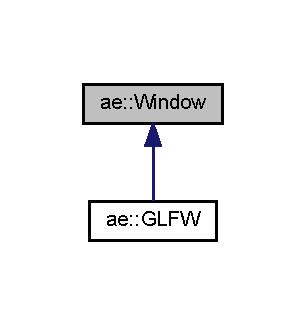
\includegraphics[width=147pt]{classae_1_1_window__inherit__graph}
\end{center}
\end{figure}
\subsection*{Public Member Functions}
\begin{DoxyCompactItemize}
\item 
\hypertarget{classae_1_1_window_aed0533cd4a633df7e42779eb3a6bafa6}{}\label{classae_1_1_window_aed0533cd4a633df7e42779eb3a6bafa6} 
{\bfseries Window} (const \hyperlink{classae_1_1_window}{Window} \&)=delete
\item 
\hypertarget{classae_1_1_window_a4cee2c65aa9028c2f540008c6d73ace0}{}\label{classae_1_1_window_a4cee2c65aa9028c2f540008c6d73ace0} 
\hyperlink{classae_1_1_window}{Window} \& {\bfseries operator=} (const \hyperlink{classae_1_1_window}{Window} \&)=delete
\item 
\hypertarget{classae_1_1_window_a27055c3b7bd792501f9fb94cc8fd898b}{}\label{classae_1_1_window_a27055c3b7bd792501f9fb94cc8fd898b} 
\hyperlink{classae_1_1_window}{Window} \& {\bfseries operator=} (\hyperlink{classae_1_1_window}{Window} \&\&)=delete
\item 
\hypertarget{classae_1_1_window_a4f08ce502de00e126f730e2121691658}{}\label{classae_1_1_window_a4f08ce502de00e126f730e2121691658} 
{\bfseries Window} (\hyperlink{classae_1_1_window}{Window} \&\&)=delete
\item 
\hypertarget{classae_1_1_window_a073b038d68804c5deeec8c9b2a9f2de2}{}\label{classae_1_1_window_a073b038d68804c5deeec8c9b2a9f2de2} 
virtual bool {\bfseries Pool\+Event} () noexcept
\item 
\hypertarget{classae_1_1_window_a64aeae1efc86ce9e502233ad8fae090b}{}\label{classae_1_1_window_a64aeae1efc86ce9e502233ad8fae090b} 
virtual std\+::vector$<$ const char $\ast$ $>$ {\bfseries extensions} () const noexcept
\end{DoxyCompactItemize}
\subsection*{Static Public Member Functions}
\begin{DoxyCompactItemize}
\item 
\hypertarget{classae_1_1_window_a2a1621593063438ea086a68fc9284997}{}\label{classae_1_1_window_a2a1621593063438ea086a68fc9284997} 
static std\+::unique\+\_\+ptr$<$ \hyperlink{classae_1_1_window}{Window} $>$ {\bfseries Create} () noexcept
\end{DoxyCompactItemize}
\subsection*{Public Attributes}
\begin{DoxyCompactItemize}
\item 
\hypertarget{classae_1_1_window_a8152047ad073d1694dbbb0d594b2138c}{}\label{classae_1_1_window_a8152047ad073d1694dbbb0d594b2138c} 
const int {\bfseries k\+Width} = 800
\item 
\hypertarget{classae_1_1_window_a7eaeaf8b679b92baa7270905b8366730}{}\label{classae_1_1_window_a7eaeaf8b679b92baa7270905b8366730} 
const int {\bfseries k\+Height} = 600
\end{DoxyCompactItemize}


The documentation for this class was generated from the following files\+:\begin{DoxyCompactItemize}
\item 
src/window.\+h\item 
src/window.\+cc\end{DoxyCompactItemize}

\hypertarget{class_window_test}{}\section{Window\+Test Class Reference}
\label{class_window_test}\index{Window\+Test@{Window\+Test}}


Inheritance diagram for Window\+Test\+:\nopagebreak
\begin{figure}[H]
\begin{center}
\leavevmode
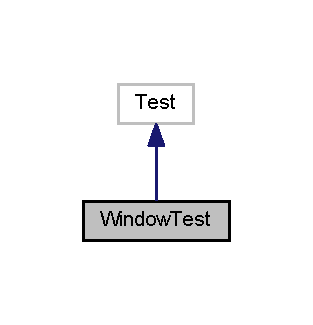
\includegraphics[width=150pt]{class_window_test__inherit__graph}
\end{center}
\end{figure}


Collaboration diagram for Window\+Test\+:\nopagebreak
\begin{figure}[H]
\begin{center}
\leavevmode
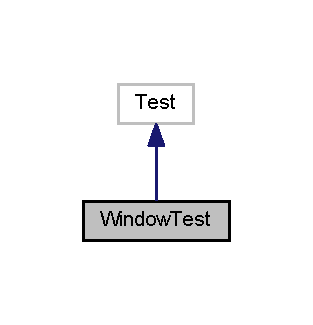
\includegraphics[width=150pt]{class_window_test__coll__graph}
\end{center}
\end{figure}
\subsection*{Protected Member Functions}
\begin{DoxyCompactItemize}
\item 
\hypertarget{class_window_test_aef877f3405cf0e40a8c7e81fe47c3a7a}{}\label{class_window_test_aef877f3405cf0e40a8c7e81fe47c3a7a} 
virtual void {\bfseries Set\+Up} ()
\end{DoxyCompactItemize}
\subsection*{Protected Attributes}
\begin{DoxyCompactItemize}
\item 
\hypertarget{class_window_test_a8c67ca4e0a784fc94b90c24a0d65ab82}{}\label{class_window_test_a8c67ca4e0a784fc94b90c24a0d65ab82} 
std\+::unique\+\_\+ptr$<$ \hyperlink{classae_1_1_window}{Window} $>$ {\bfseries window} = nullptr
\end{DoxyCompactItemize}


The documentation for this class was generated from the following file\+:\begin{DoxyCompactItemize}
\item 
src/window\+\_\+test.\+cc\end{DoxyCompactItemize}

%--- End generated contents ---

% Index
\backmatter
\newpage
\phantomsection
\clearemptydoublepage
\addcontentsline{toc}{chapter}{Index}
\printindex

\end{document}
